\documentclass[11pt,twoside, reqno, align]{amsart}
\usepackage{cancel}
\usepackage{graphicx}
\graphicspath{ {./images/} }

%%%%%%%%%%%%%%%%%%%%%%%%%%%%%%%packages%%%%%%%%%%%%%%%%%%%


%%%%%%%%%%%%%%%%%%%%%%%%%%%%%%%formatting%%%%%%%%%%%%%%%%%%

\setlength{\topmargin}{0in} 
\setlength{\oddsidemargin}{0in}   
\setlength{\evensidemargin}{0in}  
\setlength{\textheight}{8.5in}    
\setlength{\textwidth}{6.5in}  
\setlength{\headsep}{0.15in}   
\setlength{\headheight}{0in}
\parskip=4pt 

%%%%%%%%%%%%%%%%%%%%%%%%%%%%%%%formatting%%%%%%%%%%%%%%%%%%

\newtheorem{Thm}{Theorem}
\newtheorem{Def}[Thm]{Definition}
\newtheorem{Lm}[Thm]{Lemma}
\newtheorem{Prop}[Thm]{Proposition}
\newtheorem{Cor}[Thm]{Corollary}


\theoremstyle{remark}
\newtheorem{Rem}[Thm]{Remark}
\newtheorem{Exp}[Thm]{Example}
\newtheorem{Prob}{Problem}

%\numberwithin{equation}{section}



\def\R{\mathbb R}
\def\Q{\mathbb Q}
\def\N{\mathbb N}
\def\Z{\mathbb Z}
\def\P{\mathbb P}


%%%%%%%%%%%%%%%%logical connectors%%%%%%%%%%%%%%%%%%%%%%%%%%%%%%%%%%%%%

\newcommand{\OR}{\vee}
\newcommand{\AND}{\wedge}
\renewcommand{\implies}{\Rightarrow}
\newcommand{\implied}{\Leftarrow}
\renewcommand{\iff}{\Leftrightarrow}

%%%%%%%%%%%%%%%%%%%%%%%%%%%%%%%%%%%%%%%%%%%%%%%%%%%%%

\begin{document}
\title{Math 0450: Homework 2}
\date{\today}
\author{Teoh Zhixiang}

\maketitle

Use \emph{mathematical induction} to prove the following statements.

\begin{Prob}
Let $x$ be a real number, $x \neq 1$. Then, for any $n \in \N$ we have
$$
1+x+x^2+\cdots+x^n=\frac{1-x^{n+1}}{1-x}.
$$
\end{Prob}

\begin{proof}
Let $P(n)$ be defined as
$$
1+x+x^2+\cdots+x^n=\frac{1-x^{n+1}}{1-x},
$$
for $n \in \N$. Define the set $N$ as $N = \{ n \in \N \mid P(n)\}$. To prove the initial base case, we take
\begin{align*}
P(1): 1 + x^1 & = \frac{1-x^{1+1}}{1-x} \\
    1 + x & = \frac{1-x^2}{1-x} \\
    & = \frac{\cancel{(1-x)}(1+x)}{\cancel{1-x}} \quad \text{because $x \neq 1 \implies 1-x \neq 0$ } \\
    & = 1 + x
\end{align*}
Therefore $1 \in N$. Now we want to prove the statement $[P(n) \implies P(n+1)]$. If $P(n)$ is false, the statement is vacuously true. Now assume $P(n)$ is true for some $n \in \N$, that is
\begin{equation}
    P(n): 1+x+x^2+\cdots+x^n=\frac{1-x^{n+1}}{1-x},
\end{equation}
for some $n \in N$. Then to prove $P(n+1)$ true:
\begin{align*}
    1 + x + x^2 + \cdots + x^{n+1} & = 1 + x + x^2 + \cdots + x^n + x^{n+1} \\
    & = \frac{1-x^{n+1}}{1-x} + x^{n+1} \quad \text{by induction step 1} \\
    & = \frac{1-x^{n+1}}{1-x} + \frac{x^{n+1} - x^{n+2}}{1-x} \\
    & = \frac{1 - \cancel{x^{n+1}} + \cancel{x^{n+1}} - x^{n+2}}{1-x} \\
    & = \frac{1 - x^{n+2}}{1-x}.
\end{align*}
Therefore ${n+1} \in N$, and this proves $[P(n) \implies P(n+1)]$ is true. Hence $N = \N$, and $P(n)$ true.
\end{proof}

\paragraph{}

\begin{Prob}
The number of diagonals in a convex polygon with $n \geq 3$ sides equals $n(n-3)/2$.
\end{Prob}

\begin{proof}
Let $P(n)$ be defined as the statement
$$
P(n): \quad \text{number of diagonals in a convex polygon with $n$ sides} = \frac{n(n-3)}{2}
$$
for $n \in \N \setminus \{1,2\}$. Define the set $N$ as $N = \{ n \in \N \setminus \{1,2\} \mid P(n)\}$. To prove the initial base case, we take
\begin{align*}
    P(3): \quad \text{number of diagonals in a convex polygon with $3$ sides} & = \frac{3(3-3)}{2} \\
    & = \frac{3*0}{2} \\
    & = 0
\end{align*} 
Therefore $3 \in N$. Now we want to prove the statement $[P(n) \implies P(n+1)]$. If $P(n)$ is false, the statement is vacuously true. Now assume $P(n)$ is true for some $n \in \N$, that is
$$
\text{number of diagonals in a convex polygon with $n$ sides} = \frac{n(n-3)}{2}
$$
is true for some convex polygon with $n \in \N \setminus \{1,2\}$ sides. Consider an ${n+1}^{\text{th}}$ vertex added to this $n$-sided polygon that preserves the convex polygon nature of the resulting polygon. This point has to be somewhere outside the convex polygon. The picture below demonstrates this, for $n = 5$.

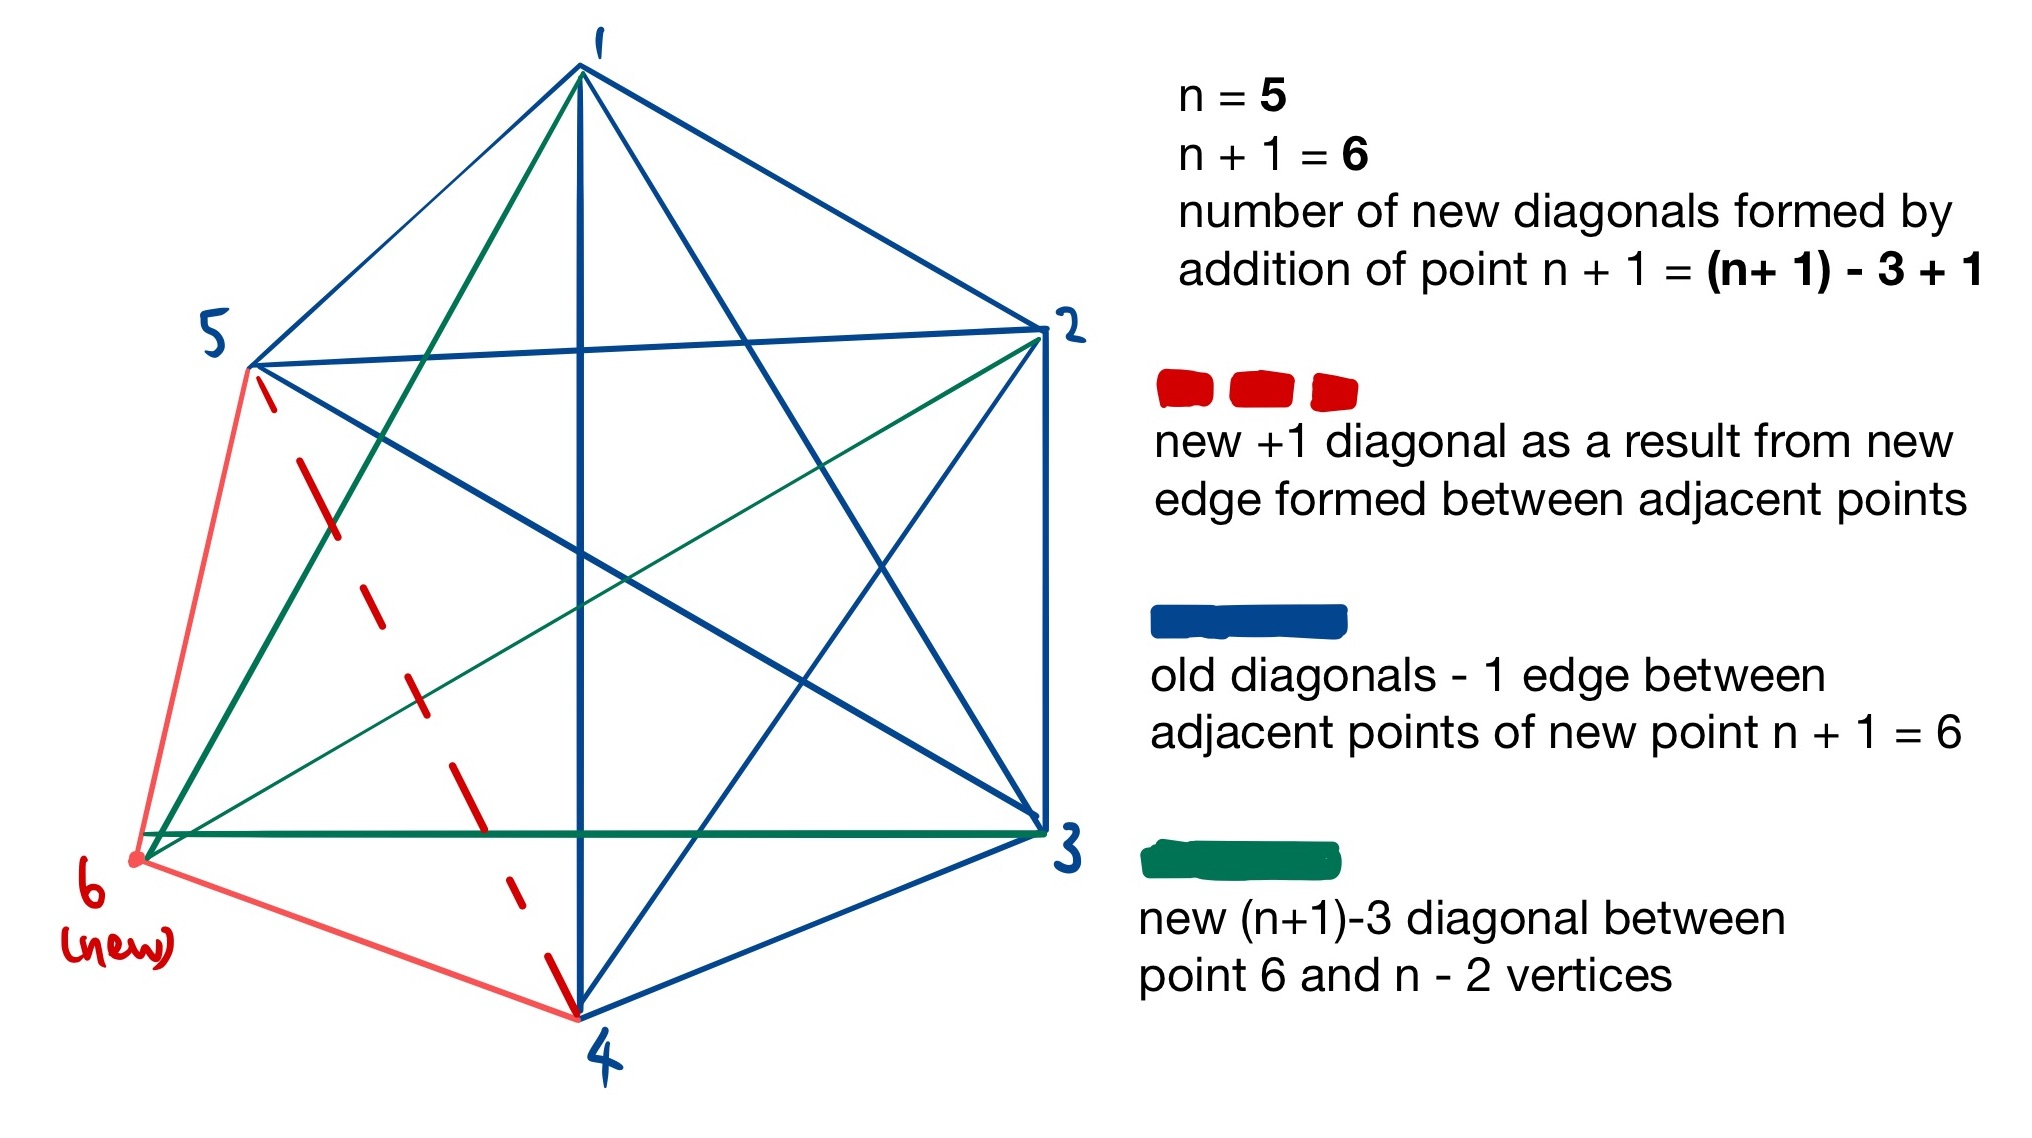
\includegraphics[scale=0.20]{math0450q2picproof.jpg}

Therefore by the combinatorial sum rule, this new point creates $((n+1)-3) + 1$ new diagonals; $(n+1)-3$ diagonals between the new ${n+1}^{\tezt{th}}$ point with the existing $(n+1)-3$ points that excludes three points, namely the ${n+1}^{\tezt{th}}$ point itself and its two adjacent points, and $1$ additional diagonal that is the edge between its two adjacent points. As a result we have
\begin{align*}
    \text{number of diagonals in a convex polygon with $n+1$ sides} & = \frac{n(n-3)}{2} + ((n+1)-3) + 1 \\
    &\quad \text{(using induction step $P(n)$} \\
    &\quad \text{and number of new diagonals)} \\
    & = \frac{n(n-3)}{2} + n - 1 \\
    & = \frac{n(n-3)}{2} + \frac{2(n-1)}{2} \\
    & = \frac{n^2-3n+2n-2}{2} \\
    & = \frac{n^2-n-2}{2} \\
    & = \frac{(n+1)(n-2)}{2} \\
    & = \frac{(n+1)((n+1)-3)}{2}
\end{align*}
which shows ${n+1} \in N$, and this proves $[P(n) \implies P(n+1)]$ is true. Hence $N = \N \setminus \{1,2\}$, and $P(n)$ true.
\end{proof}

\paragraph{}

\begin{Prob}[Prime factorization]
Any natural number greater than $1$ can be written as a product of prime numbers and/or $1$.
\end{Prob}

\begin{proof}
% Now we want to prove the statement $[P(3) \AND P(4) \AND P(5) \AND \cdots \AND P(n) \implies P(n+1)]$ (Principle of Strong Induction). If the antecedent is false, the statement is vacuously true. Now assume $P(3) \AND P(4) \AND P(5) \AND \cdots \AND P(n)$ is true, that is

Define the set of prime numbers $\P$ as
$$
\P = \{p \in \N \mid p \text{ is prime}\}
$$

Let $P(n)$ be defined as the statement
$$
P(n): \quad n = a*b,
$$
for $n \in \N \setminus \{1\}$, $a,b \in \P \cup \{1\}$ or [$(a\text{ product of primes}) \OR (b\text{ product of primes})$]. 

Define the set $N$ as $N = \{ n \in \N \setminus \{1\} \mid P(n)\}$. To prove the initial base case, we take
$$
P(2): \quad 2 = 2*1,
$$
where $2 \in \P \cup \{1\}$, and so $2 \in N$. Next we want to prove the statement $[(P(2) \AND P(3) \AND P(4) \AND P(5) \AND \cdots \AND P(n)) \implies P(n+1)]$ (Principle of Strong Induction). If the antecedent is false, the statement is vacuously true. Now assume $P(2) \AND P(3) \AND P(4) \AND P(5) \AND \cdots \AND P(n)$ is true, that is that $P(n)$ is true for all natural numbers $1 < k \leq n$. Then we want to prove $P(n+1)$ true. Consider two cases: if $n+1 \in \P$ then $n+1 = (n+1)*1$, and $P(n+1)$ is true. If $n+1 \not\in \P$, then because $n+1 > 2$ we have
$$
n+1 = u*v,
$$
where $1 < u,v < n+1 \in \N$. Note that above we assumed $P(2) \AND P(3) \AND P(4) \AND P(5) \AND \cdots \AND P(n)$ is true. Therefore any $u, v < {n+1} \in N$ are individually primes or products of primes; consequently $n+1 = u*v$ is also product of primes. $n+1 \in N$, and thus $P(n+1)$ is true. Since we have proven strong inductive step $[(P(2) \AND P(3) \AND P(4) \AND P(5) \AND \cdots \AND P(n)) \implies P(n+1)]$, we have proven $P(n) \in N$: all natural numbers greater than $1$ can be written as primes or products of primes and/or $1$.
\end{proof}

\paragraph{}

\begin{Prob}[Binary expansion]
Any $n\in \N$ can be written as 
$$
n=c_k2^k+c_{k-1}2^{k-1}+\cdots+c_02^0,
$$
for some $k\in \N_*$ and $c_i\in\{0,1\}$, $0\leq i\leq k$.
\end{Prob}

\begin{proof}
% To prove this statement we use the following $Lemma$:

% [$Problem$ 1]. Let $x$ be a real number, $x \neq 1$. Then, for any $n \in \N$ we have
% $$
% 1+x+x^2+\cdots+x^n=\frac{1-x^{n+1}}{1-x}.
% $$
% We then derive the following corollary:

% [Corollary]. Set $x = 2 \neq 1$:
% \begin{align*}
%     1+2+2^2+\cdots+2^k & = \frac{1-2^{k+1}}{1-2} \\
%     & = 2^{k+1}-1
% \end{align*}
% for all $k \in \N$. Applying this result to $2^k$ we see that every $2^{k}$ can be written as

% \begin{align*}
%     2^k & = 1 + 2 + 2^2 + \cdots + 2^{k-1} + 1 \\
%     & = \mathbf{1} + (\mathbf{1} + 1) + (\mathbf{1} + 2 + 1) + \cdots + (\mathbf{1} + 2 + 2^2 + \cdots + 2^{k-2} + 1) + 1 \\
%     & = \underbrace{\mathbf{1} + \mathbf{1} + \cdots + \mathbf{1}}_\text{$2^{k-1}$ terms} + 2 + 2 + \cdots + 2 + 2^2 +\cdots + 2^2 + 2^{k-2} + 1 + 1 + \cdots + 1
% \end{align*}
% This means that every natural number $n$ between any two orders of $2$ can be expressed as in terms of a series of orders of $2$. This is shown as follows:
% \begin{align*}
%     2^{k-1} & = \frac{2^k}{2} \\
%     & = 2^k - 2^{k-1} \\
%     & = 2^k - (\underbrace{\mathbf{1} + \mathbf{1} + \cdots + \mathbf{1}}_\text{$2^{k-1}$ terms})
% \end{align*}
% This proves the Binomial expansion theorem.
% Take note that the corollary we derived initially was defined for all $k \in \N$. This left out the case when $k = 0$, i.e. $2^{0+1} - 1 = 2^0$. Let's show that this particular case when $k = 0$ also satisfies the Binary expansion statement in $Problem$ 4; i.e. when $n = 1$ and $n = 2$:
% \begin{align*}
%     n &= 1 = 1(2^0) \quad \text{and} \\
%     n & = 2 = 0(2^0) + 1(2^1)
% \end{align*}
Let $P(n)$ be the statement that $n \in \N$ can be written as
$$
n=c_k2^k+c_{k-1}2^{k-1}+\cdots+c_02^0,
$$
for some $k \in \N_*$ and $c_i \in \{0,1\}$, $0 \leq i \leq k$. Define the set $N$ as $N = \{ n \in \N \mid P(n)\}$. First we show $P(0)$ true:
$$
0 = 0 \cdot 2^0
$$
and so $0 \in N$, $P(0)$ true. Next we assume that $P(n)$ true for all $n \geq 0$ (Principle of Strong Induction). We need to show $P(n+1)$ true as a result. Consider two cases: $n+1$ even and $n+1$ odd. If $n+1$ even, then $\frac{n+1}{2} \leq n \in \N$, and so by inductive step
$$
\frac{n+1}{2} = c_k2^k+c_{k-1}2^{k-1}+\cdots+c_02^0.
$$
Consequently 
\begin{align*}
   n+1 & = c_k2^{k\mathbf{+1}}+c_{k-1}2^{k-1\mathbf{+1}}+\cdots+c_02^{0\mathbf{+1}} \\
   & = c_k2^{k+1}+c_{k-1}2^k+\cdots+c_02^1 + 0\cdot2^0.
\end{align*}
If $n+1$ odd, then $n \in \N$ must be even, i.e.
\begin{align*}
    \frac{n}{2} & =c_k2^k+c_{k-1}2^{k-1}+\cdots+c_02^0 \\
    n & = c_k2^{k+1}+c_{k-1}2^k+\cdots+c_02^1
\end{align*}
and therefore we can surely also represent $n+1$ as a binary representation:
\begin{align*}
    n+1 & = c_k2^{k+1}+c_{k-1}2^k+\cdots+c_02^1 + 1\cdot2^0,
\end{align*}
proving $n+1 \in N$. And so we have proven the binary expansion theorem for all $n \in \N$.
\end{proof}

\paragraph{}

\begin{Prob}[Cauchy-Schwarz inequality]
For any $n\in \N$ and real numbers $a_i$, $b_i$, $1\leq i\leq n$ we have 
$$
|a_1b_1+a_2b_2+\cdots+a_nb_n|\leq (a_1^2+a_2^2+\cdots+a_n^2)^{1/2}(b_1^2+b_2^2+\cdots+b_n^2)^{1/2}.
$$
\end{Prob}

\begin{proof}
Proof by induction. Let $P(n)$ be defined as
$$
|a_1b_1+a_2b_2+\cdots+a_nb_n|\leq (a_1^2+a_2^2+\cdots+a_n^2)^{1/2}(b_1^2+b_2^2+\cdots+b_n^2)^{1/2}7,
$$
for $n \in \N$ and real numbers and real numbers $a_i$, $b_i$, where $1\leq i\leq n$. We shall prove two base cases $P(1)$ and $P(2)$, then prove the inductive step $P(n) \implies P(n+1)$. Define the set $N$ as $N = \{ n \in \N \mid P(n)\}$. 

Base cases:
\begin{align*}
    P(1): \quad |a_1b_1| & \leq (a_1^2)^{1/2}(b_1^2)^{1/2} \\
    (a_1^2)^{1/2}(b_1^2)^{1/2} & = (a_1^2b_1^2)^{1/2} \\
    & = (a_1b_1)^{2(1/2)} \\
    & = +a_1b_1 \\
    & = |a_1b_1| \\
    & \geq |a_1b_1|
\end{align*}
so $1 \in N$. And
\begin{align*}
    P(2): \quad |a_1b_1 + a_2b_2| & \leq (a_1^2 + a_2^2)^{1/2}(b_1^2 + b_2^2)^{1/2} \\
    % (a_1^2 + a_2^2)^{1/2}(b_1^2 + b_2^2)^{1/2} & = ((a_1^2 + a_2^2)(b_1^2 + b_2^2))^{1/2} \\
    % & = (a_1^2b_1^2 + a_1^2b_2^2 + a_2^2b_1^2 + a_2^2b_2^2)^{1/2} \\
    & \text{(square both sides)} \\
    (a_1b_1 + a_2b_2)^2 & \leq  (a_1^2 + a_2^2)(b_1^2 + b_2^2) \\
    a_1^2b_1^2 + a_2^2b_2^2 + 2a_1b_1a_2b_2 & \leq a_1^2b_1^2 + a_2^2b_2^2 + a_1^2b_2^2 + a_2^2b_1^2 \\
    \text{to show:} \\
    2a_1b_1a_2b_2 & \leq a_1^2b_2^2 + a_2^2b_1^2 \\
    0 & \leq a_1^2b_2^2 + a_2^2b_1^2 - 2a_1b_1a_2b_2 \\
    0 & \leq (a_1b_2 - a_2b_1)^2
\end{align*}
so $2 \in N$. Next we assume $P(n)$ true for some $n \in \N$. Then to prove $P(n+1): |a_1b_1+a_2b_2+\cdots+a_{n+1}b_{n+1}| \leq (a_1^2+a_2^2+\cdots+a_{n+1}^2)^{1/2}(b_1^2+b_2^2+\cdots+b_{n+1}^2)^{1/2}$ true:
\begin{align*}
    |a_1b_1+a_2b_2+ \cdots +a_{n+1}b_{n+1}| & = |(a_1b_1+a_2b_2+ \cdots +a_nb_n) + a_{n+1}b_{n+1}| \\
    % & \leq |a_1b_1+a_2b_2+ \cdots +a_nb_n| + |a_{n+1}b_{n+1}| \\
    & \leq |(a_1^2+a_2^2+\cdots+a_n^2)^{1/2}(b_1^2+b_2^2+\cdots+b_n^2)^{1/2} + a_{n+1}b_{n+1}| \\
    & \text{let $(a_1^2+a_2^2+\cdots+a_n^2)^{1/2} = A$ and $(b_1^2+b_2^2+\cdots+b_n^2)^{1/2} = B$} \\
    & \overbrace{\leq} |AB + a_{n+1}b_{n+1}| \\
    & \overbrace{\leq}^\text{by $P(2)$} (A^2 + a_{n+1}^2)^{1/2}(B^2 + b_{n+1}^2)^{1/2} \\
    & = (a_1^2+a_2^2+\cdots+a_n^2 + a_{n+1}^2)^{1/2}(b_1^2+b_2^2+\cdots+b_n^2 + b_{n+1}^2)^{1/2} \\
\end{align*}
and so $n+1 \in N$. Therefore by Principle of Mathematical Induction, $N = \N$, and $P(n):= \text{Cauchy-Schwarz Inequality}$ is true for all $n \in \N$.
\end{proof}

\end{document}